% !TEX root = Monografia Mestrado.tex

\chapter{Análise do cenário atual}
\label{Cap:analise:cenario}

\section{Análise Organizacional e de Processos}
\label{Sec:analise:org}

\textbf{Diagnóstico:} observou-se que a empresa possui qualidades essenciais para o crescimento contínuo, como por exemplo, o comprometimento dos profissionais, a comunicação, o bom clima organizacional, assim como a cultura de prezar pela excelência e ser reconhecida através da sua confiabilidade e qualidade nos serviços. Porém, para que a empresa suporte o crescimento que tende a acontecer cada vez mais, devido a demanda pelos serviços, torna-se necessário alguns reajustes nos processos.

\subsection{Suporte Técnico}
\label{Sec:suporte}

Este departamento é o único responsável pelo atendimento ao cliente atualmente. Assuntos sobre problemas e dúvidas relacionados aos \sws fornecidos são tratados diretamento com os técnicos do suporte. Para isso o departamento se utiliza de 2 \sws, cujas especificações estão relacionadas na Tabela \ref{Tab:espec:sw:atend} e as janelas principais podem ser observadas nas Figuras \ref{Fig:jan:contatos:lanca} e \ref{Fig:jan:pendencias:lanca}.

\begin{table}[h!]\footnotesize
\centering
\begin{tabular}
{
 	|p{1,5cm}|p{12cm}|
}

	\hline
	\textbf{Nome}&
	\textbf{Especificações}\\
	\hline

	Contatos&
	\begin{itemize}
	\item Registra atendimentos;
	\item Registra o cliente que está sendo atendido;
	\item Possui um espaço virtualmente ilimitado para informar o assunto do contato;
	\item Cronometra automaticamente o atendimento;
	\item Possui uma data de previsão de retorno;
	\item Não permite inclusões de novas interações com o cliente durante o andamento do atendimento, que pode se extender por dias (neste caso novos atendimentos deverão ser registrados, sem haver qualquer ligação entre a primeira e as demais chamadas).
	\end{itemize}\\
	\hline

	Pendências&
	\begin{itemize}
	\item Registra tarefas;
	\item Registra o cliente que fez a solicitação (opcional);
	\item Associa o solicitante e o responsável por sua realização (ambos colaboradores da empresa);
	\item Permite definir prioridade, data limite para realização e previsão de atendimento;
	\item Possui um controle de fechamento, onde o responsável indica a data em que aquela tarefa foi realizada;
	\item Possui um controle de ``ok'', onde o solicitante indica que aquela tarefa já foi liberada para o cliente;
	\item Diferentemente do Contatos, permite acrescentar novas tarefas ao mesmo registro principal.
	\end{itemize}\\
	\hline
	
\end{tabular}
\caption {Especificações dos \sws de atendimento}
\label{Tab:espec:sw:atend}
\end{table}

\begin{figure}[!h]
\centering
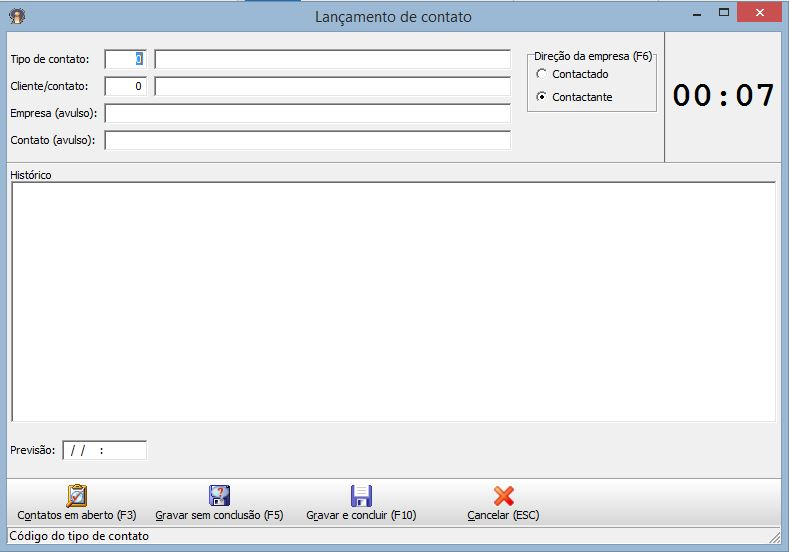
\includegraphics[scale=0.6]{figuras/jan_contatos_lancamento.jpg}
\caption{Janela de lançamento dos atendimentos}
\label{Fig:jan:contatos:lanca}
\end{figure}

\begin{figure}[!h]
\centering
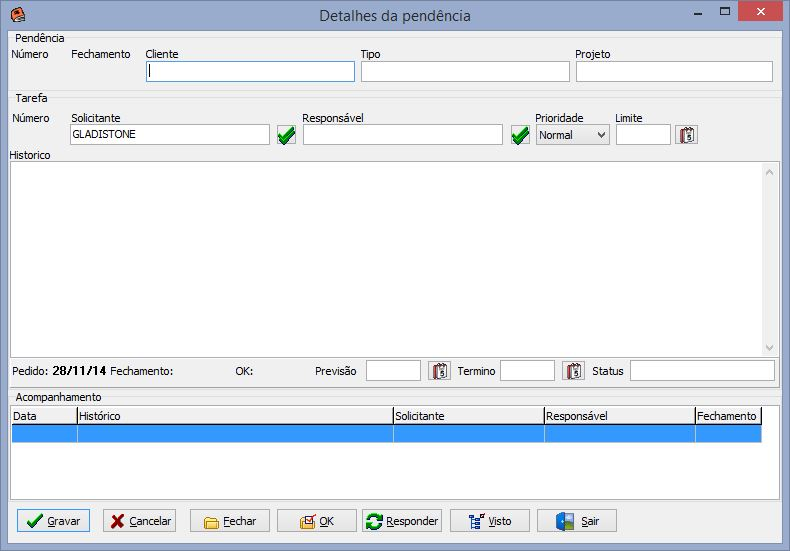
\includegraphics[scale=0.6]{figuras/jan_pendencias_lancamento.jpg}
\caption{Janela de lançamento das pendencias}
\label{Fig:jan:pendencias:lanca}
\end{figure}

Os atendimentos podem ser realizados através do telefone, acesso remoto via internet, e-mail ou presencial. Como pode ser observado na Figura \ref{Fig:atend11}, somente 3 tipos foram registrados no mês de novembro de 2014, mostrando que as comunicacões via e-mail não são registradas.

\begin{figure}[!h]
\centering
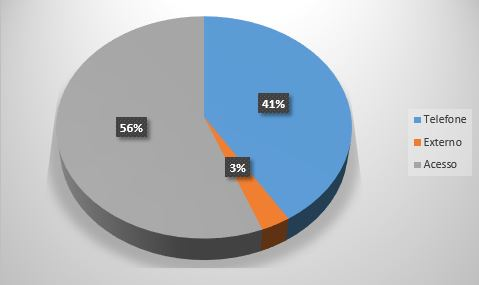
\includegraphics[scale=0.5]{figuras/atendimentos_por_tipo.jpg}
\caption{Atendimentos por tipo em novembro/2014}
\label{Fig:atend11}
\end{figure}

Outros problemas foram diagnosticados e estão relacionados na Tabela \ref{Tab:probl:atend}, sendo a falta de acompanhamento do andamento das solicitações e retorno ao cliente as mais críticas.

\begin{table}[h!]\footnotesize
\centering
\begin{tabular}
{
 	|p{14cm}|
}

	\hline
	\textbf{Problema diagnosticado}\\
	\hline

	Falta de registro de atendimento (para qualquer tipo)\\
	\hline

	Postergação de registro de atendimento (para qualquer tipo), que pode levar ao esquecimento (falta de registro)\\
	\hline
	
	Dados insuficientes sobre o contato\\
	\hline
	
	 Falta de acompanhamento do andamento das solicitações (fechamento dos registros de atendimento)\\
	\hline

	 Falta de retorno da situação das solicitações ao cliente\\
	\hline

	Tarefas originadas dos atendimentos, para o próprio departamento de suporte ou para outros departamentos, são registradas em um \sw separado e não há nenhuma rastreabilidade\\
	\hline

\end{tabular}
\caption {Problemas diagnosticados no departamento de suporte}
\label{Tab:probl:atend}
\end{table}

As seguintes ações devem ser tomadas para contonar os problemas diagnosticados:

\begin{itemize}

\item Todos os chamados técnicos deverão ser registrados no ato de sua execução (ligação, acesso remoto ou recebimento do e-mail), com exceção do atendimento externo que deve ser registrado no ato do retorno do técnico;

\item O máximo de informações possíveis precisa ser registrado no histórico do chamado;

\item A fusão entre o Contatos e o Pendências é extremamente necessária, a fim de criar um registro de todas as ações vinculadas naquele chamado, tornando-se obrigatório o registro de todas as ações realizadas por cada técnico que atender o chamado;

\item Qualquer nova informação de um chamado deve ser adicionada ao registro já aberto, sem a necessidade de abrir um novo chamado e permitindo a rastreabilidade;

\item Um departamento de Serviço de Atendimento ao Cliente (SAC) deverá ser criado e pelo menos uma pessoa deve ser colocada como responsável pelas suas atribuições;

\item O SAC realizará o fechamento do chamado junto ao cliente, consultando se realmente o problema foi solucionado e realizando pesquisas de satisfação e gerando indicadores de desempenho e qualidade (tempo médio de conclusão dos chamados, problemas mais ocorridos, cliente mais ativo, técnico mais ativo, etc);

\item Os clientes deverão receber um Documento de Abertura e Acompanhamento de Chamados, juntamente com o manual  do \sw, para que saibam exatamente como proceder para abrir e acompanhar um chamado;

\item Para uma melhor performance da equipe de suporte, deverá ser feito a gestão do conhecimento, documentando a resolução de cada problema que surja no atendimento do suporte técnico;

\item É necessária a elaboração de um fluxograma do atendimento, com as informações chaves de requisitos para abertura de chamados;

\item É necessária a elaboração de um fluxograma do atendimento de serviços diferenciados, tais como treinamentos, suportes avulsos, entrada de equipamento para concerto ou manutenção, entre outros, lembrando de acrescentar no fluxo a emissão da Ordem de Serviço;

\item Deverá ser realizado o acompanhamento dos clientes que não abrem chamado com o suporte há mais de 3 meses.

\end{itemize}

\subsection{Desenvolvimento}
\label{Sec:desenvolvimento}

Este departamento não tem contato direto com os clientes, pois todas as solicitações passam pelo departamento de suporte técnico. Porém, todas as solcitações de mudança ou correção de problemas nos \sws são resolvidas por este departamento e alguns atendimentos são repassados para o setor de desenvolvimento para resolução conjunta quando os técnicos não possuem conhecimento ou capacidade para tratá-los por si mesmos. 

As tarefas deste departamento são registradas no \sw Pendências mas, como já relatado anteriormente, não possuem relacionamento com os chamados abertos no \sw Contatos. Todos os problemas diagnosticados estão relacionados na Tabela \ref{Tab:probl:desenv}.

\begin{table}[h!]\footnotesize
\centering
\begin{tabular}
{
 	|p{14cm}|
}

	\hline
	\textbf{Problema diagnosticado}\\
	\hline

	Falta de posicionamento quanto ao andamento das solicitações\\
	\hline

	Falta de previsão de entrega das soluções\\
	\hline

	Falta de rastreabilidade entre abertura de chamados e tarefas\\
	\hline

\end{tabular}
\caption {Problemas diagnosticados no departamento de desenvolvimento}
\label{Tab:probl:desenv}
\end{table}

Para solucionar os problemas diagnosticados para este setor, além das ações ja citadas em \ref{Sec:suporte}, serão necessárias as seguintes ações:

\begin{itemize}

\item Criar processos para determinar a previsão de lançamento de versões de \sws;

\item Criar processos para determinar em qual versão determinada solicitação será incluída;

\item Integrar aos \sws de atendimento as informações de lançamento de versões e, consequentemente, a previsão das solicitacões.

\end{itemize}

\subsection{Financeiro}

O departamento financeiro lida com o cliente com uma frequência menor que os departamentos de suporte e desenvolvimento. Porém, os assuntos relacionados a este departamento podem gerar transtornos e prejuízos quando feitos de forma incorreta. Além disso, este departamento também é responsável por bloquear o atendimento aos clientes inadimplentes, portanto representa um papel importante nos processos descritos em \ref{Sec:suporte} e \ref{Sec:desenvolvimento}.

Nenhum atendimento ou tarefa relacionados a este departamento são registrados nos \sws de atendimento. Portanto, as ações necessárias para melhoria dos processos são:

\begin{itemize}

\item Registrar todo e qualquer contato com clientes nos \sws de atendimento;

\item Integrar as informações financeiras com os \sws de atendimento para que a liberação ou bloqueio seja feito automaticamente no ato da identificação do cliente.

\end{itemize}

\subsection{Marketing}

O departamento de marketing é o responsável, geralmente, pelo primeiro contato com o cliente. Durante as negociações de venda de \sw, é comum haver solicitações de modificações ou acertos sobre configurações, conversões de dados e treinamentos. Porém, nenhuma dessas informações são registradas nos \sws de atendimento. O mesmo ocorre na venda de equipamentos e outros serviços.

Portanto, as ações necessárias para melhoria dos processos são:

\begin{itemize}

\item Registrar os primeiros contatos com todos os prospectos, mesmo que não se tornem clientes;

\item Registrar toda e qualquer interação com os clientes, novos ou antigos;

\item Incluir nos registros as informações sobre negociação, possíveis modificações, conversões e outras condições estabelecidas durante ou após a venda.

\end{itemize}

\section{Análise SWOT}

A fim de resumir e melhor entender a análise organizacional e de processos realizada em \ref{Sec:analise:org}, foi desenvolvida a Tabela \ref{Tab:SWOT} com a análise SWOT.

\begin{table}[h!]\footnotesize
\centering
\begin{tabular}
{
	| >{\centering\arraybackslash}p{7cm}
	| >{\centering\arraybackslash}p{7cm}|
}
\hline

	Forças&
	Fraquezas\\
	\hline

	%Forças
	\begin{tabular}{p{6,8cm}}
	Comprometimento dos profissionais;\\
	Bom clima organizacional;\\
	Cultura de prezar pela excelência;\\
	Ser reconhecida através da sua confiabilidade e qualidade nos serviços.\\
	\end{tabular}&

	%Fraquezas
	\begin{tabular}{p{6,8cm}}
	Falta de informações no acompanhamento de solicitações;\\
	Ineficiência na comunicação com o cliente.\\
	\end{tabular}\\
	\hline

	Oportunidades&
	Ameaças\\
	\hline

	% Oportunidades
	\begin{tabular}{p{6,8cm}}
	Taxa de crescimento elevada nos últimos meses;\\
	Aumento no faturamento;\\
	Alta divulgação da marca, dentro e fora da sua própria cidade.\\
	\end{tabular}&

	% Ameaças
	\begin{tabular}{p{6,8cm}}
	Perder a confiabilidade dos clientes;\\
	Manchar a reputação;\\
	Sofrer queda nas vendas pela perda de indicações de clientes e parceiros insatisfeitos;\\
	Sofrer perda de clientes já estabelecidos por não prestar um bom atendimento.\\
	\end{tabular}\\
	\hline

\end{tabular}
\caption {Análise SWOT dos processos}
\label{Tab:SWOT}
\end{table}